\documentclass[preprintnumbers,amsmath,amssymb,prd,superscriptaddress,notitlepag
e, twocolumn]{revtex4-1}
\pdfoutput=1

\usepackage{graphicx}% Include figure files
\usepackage{dcolumn}% Align table columns on decimal point
\usepackage{bm}% bold math


\newcommand{\OmegaDE}{\Omega_{\rm DE}}
\newcommand{\rhoDE}{\rho_{\rm DE}}
\def\as#1{[\textbf{AS}: \textit{#1}] }

\begin{document}

\title{Early Dark Energy: Reality and Fiction}

\author{Jose Vazquez}
\email{jvazquez@bnl.gov}
\affiliation{Brookhaven National Laboratory, Upton, NY 11973, USA}
\author{An\v{z}e Slosar}
\email{anze@bnl.gov}
\affiliation{Brookhaven National Laboratory, Upton, NY 11973, USA}
\author{David H. Weinberg}
\email{dhw@astronomy.ohio-state.edu}
\affiliation{Center for Cosmology and Astro-Particle Physics, Ohio State University, Columbus, Ohio, USA}
\affiliation{Department of Astronomy, Ohio State University, Columbus, Ohio, USA}
\date{\today}

\begin{abstract}
  Early dark energy is an attractive to solution to several conundrums
  associated with the current epoch of accelerate expansion of the
  Universe. While significant amounts of early dark energy have been
  ruled out by several papers, a curious degeneracy was noted in
  Auburg et al 2015.  When considering expansion history data alone, a
  surprising large amounts of early dark energy are consistent with
  the $\Omega_m h^2$ and $D_a/r_s$ determined by the CMB and a
  compendium of low-redshift expansion history data. Although
  seemingly at odds with results that included perturbations, it
  seemed to be a promising path toward alleviating Hubble parameter
  and perturbation amplitude tensions.  In this paper we investigate
  this degeneracy further, by solving exact scalar field equations,
  instead of using an imposed variation of the equation of state. We
  find that the degeneracy in realistic scalar field approximately
  holds, but that it is very significantly broken by the precise
  background data. We note that realistic scalar field models contain
  large transients between matter and radiation tracking and therefore
  caution against usage of oversimplified models of early dark energy.
  
\end{abstract}

\maketitle

\section{Introduction} 
 In typical cosmological models, dark energy is dynamically negligible
 at high redshifts because its energy density is assumed independent
 (or weakly varying) with the scale factor. However, some scalar field
 potentials yield a dark energy density that tracks the energy density
 of the dominant species during the radiation and matter dominated
 eras, then asymptotes towards a cosmological constant at late times.
 These models ameliorate, to some degree, the ``coincidence problem"
 of constant-$w$ models because the ratio of dark energy density to
 total energy density varies over a much smaller range.
 
 In Auburg et al 2015, an extensive study of various cosmological
 constraints that can be derived by consideration of background history
 has been performed. In particular in the section of dark energy, the
 analysis has been done using the Doran-Robbers model (cite), which
 postulates that the dark energy energy density varies with the
 cosmological scale factor $a$ as
 \begin{equation}
\OmegaDE(a) = {\OmegaDE - \OmegaDE^e\left(1-a^{-3w_0}\right)
               \over \OmegaDE + \Omega_m a^{3w_0}}
			   + \OmegaDE^e\left(1-a^{-3w_0}\right)~,
 \label{eqn:ede}
 \end{equation}
 This functional form effectively parameterizes the dark energy
 through three parameters $\OmegaDE$ (the energy density in the dark
 energy today), $\OmegaDE^e$ (the energy density in the dark energy at
 early times) and the $w_0$ the equation of state of energy density
 today. This form implies a certain equation of state parameter which
 is such that the dark energy exhibits tracking behavior: it tracks
 the evolution of dark matter in the early universe.

 In Auburg et a al 2015, it has been found that this particular form
 exhibit strong degeneracy, when considering just background
 quantities. Namely, when CMB data are compressed into measurements of
 $\Omega_mh^2, \Omega_bh^2 and D_a(z=1150/r_s)$ and one combined with
 low-redshift Baryon Acoustic Oscillations (BAO) and supernova-Ia (SN)
 data, large amounts of early dark energy are consistent with the
 data, up to $\OmegaDE^e$ of 0.4. This behavior has been tracked to
 the perfect tracking of the dominant component by the early dark
 energy, which allows quantities to match perfectly upon a small
 rescaling of the $z=0$ Hubble parameter $H_0$. \as{Expand this
   section}. 

 The purpose of this paper is to study this phenomenon in greater
 detail. In particular, we are interested to understand if this
 behavior is still present in more realistic scalar-field models and
 if it can simultaneously alleviate tensions in $H_0$ and
 $\sigma_8$ that are present between CMB and low-redshift data. This
 already assumes that tensions with perturbations could be alleviated
 using some other mechanism. We find, however, that no, the large
 degeneracy is an artifact of a perfect tracking that is not present
 in realistic scalar-field models that the simplified Doran-Robbers
 model was supposed to emulate.

 \section{Early dark energy models}
 We study two early dark-energy models. The first one is the
 Doran-Robbers (DR) model, which specifies the evolution of dark
 energy density with redshift as prescribed in the equation
 \ref{eqn:ede}.

 The second one is the more realistic scalar field model. The
 evolution equations for a scalar field are given by
 \begin{eqnarray}\label{eq:hub}
   \ddot \phi &+&3H\dot \phi + V_{\phi} = 0, \\
   H^2 &=& \frac{8\pi G}{3} \left[ \frac{1}{2}{\dot \phi}^2 + V(\phi) +\rho  \right],
 \end{eqnarray}
 and its corresponding equation of state is given by 
 \begin{equation}
   w = \frac{ \frac{1}{2}{\dot \phi}^2 -V(\phi) }{ \frac{1}{2}{\dot \phi}^2 +V(\phi)}. 
 \end{equation}
 In this paper we consider a particular functional form for $V(\phi)$
 given in a seminar paper by Albrecht and Skordis (AS):
 \begin{equation}
   V(\phi)=V_0[(\phi -B)^2+A]\exp(-\lambda \phi)
 \end{equation} 

 From now on, we refer to the two models as DR and AS model
 respectively.
 
\section*{Tuning Albrech-Skordis model}

In AS model, $A, B$ and $\lambda$ are free parameters; $V_0$ is fixed such
that the density parameter $\Omega_{\phi}$ today takes the value of
the Dark energy. It is common to parameterize this model using the set
$\{A, A\lambda^2,B\}$.  Figure \ref{fig:fig1}, shows three components of the
universe: radiation (yellow), dark matter (green) and Early Dark
energy for different set of parameter combinations.   Notice, from the
middle panel that the factor $A\lambda^2$ only affects the future of
the universe with no effect to the past, and hence does not affect the
observational constraints.

\textbf{
A number of questions:}
\begin{itemize}
\item Why is $w$ -1 at early times rather than $1/3$ for radiation
  tracking?
\item Can you make the same plot for Doran model
\item Can you mark the matter-radiation redshift on these plots?
\item Let's not go that far into the future, stop at ln a = 1
\end{itemize}


\begin{figure*}[h!]
\hspace*{-0.in}
 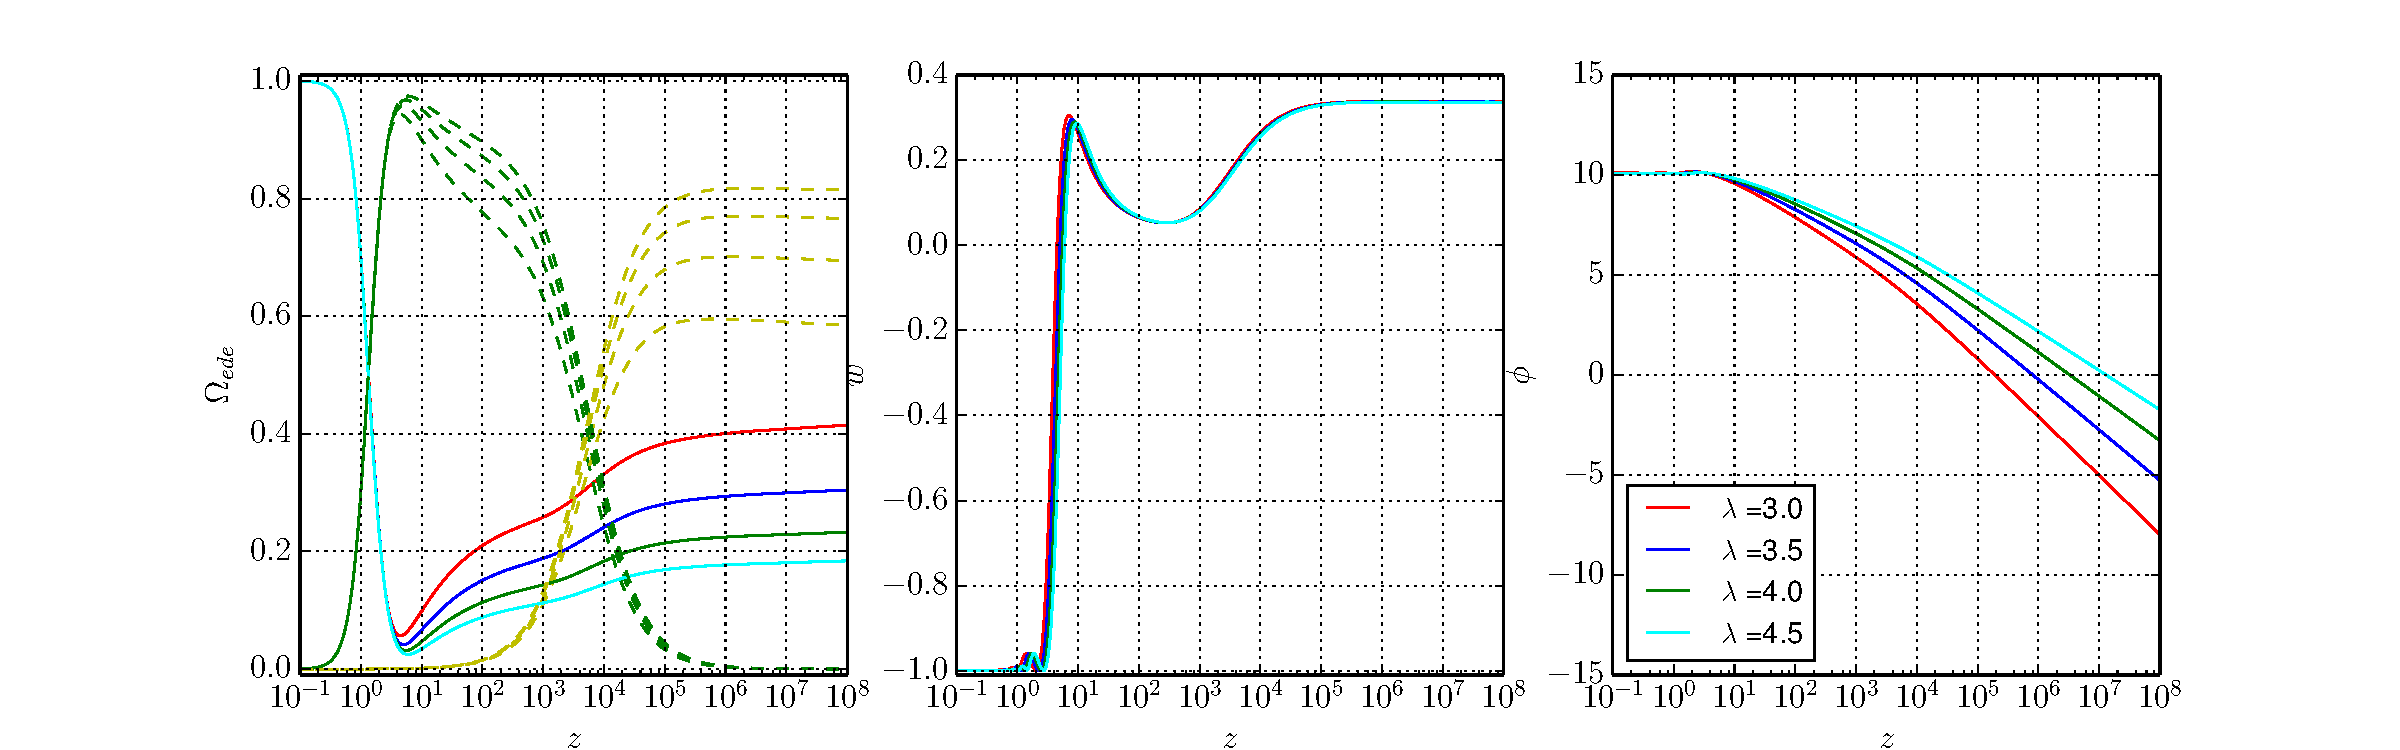
\includegraphics[trim = 2mm 2mm 3mm 1mm, clip, width=20cm, height=5.5cm ]{Quint_vl_phi.pdf}
 \caption{  Three components of the universe: radiation (yellow), dark matter (green) 
 and Early Dark energy for different set of parameter combinations.
Density parameters (left), equation of state (middle) and the scalar
field (right) in terms of the $\ln(a)$ scale factor.
\as{Make sure these plots are actually readable. Can't see the labels
  at all!}
 }
 \label{fig:fig1}
\end{figure*} 



\section{Expansion history degeneracy}


We now study the expansion history degeneracy. For each chosen
$\OmegaDE^E$ and early dark energy model considered (DR or AS), we fix
$\Omega_mh^2$ and $\Omega_bh^2$ to their CMB-determined values. We
then adjust the Hubble parameter in order to match $D_A/r_s$ at
$z=1150$, to match the CMB peak positions measured by Planck. This
completely determines the background evolution; the question now is
whether these points go through low-redshift data. 

Now need to replot the plots
\begin{itemize}
\item The plots should be the same for DR and for AR
\item For both plot $D_a/r_s$ and $D_h/r_s$ as now
\item Then, on the same plot, as a function of $\OmegaDE^e$, plot
  $\Omega_m/\Omega_{mf}$, $H_0/H_{0f}$, $\sigma_8/\sigma_{8f}$,
  $r_s/r_{sf}$ where $f$ is fiducial (i.e. $\Lambda$CDM,
  $\OmegaDE^e=0$).
\item On this plot, you can also plot the ``prediction''
  $r_s=r_{sf}\sqrt{1-\OmegaDE^e}$ or whatever.
\end{itemize}




 


We see from Figure \ref{fig:fig1} that $r_s \propto (1-\Omega_{\rm ede})^{1/2}$ up to 0.2\%
for $\Omega_{ede}=0.08$, and the observables $D_A(z)/r_d $ and $D_H(z)/r_d$ satisfy 
 BAO observations from both Galaxies and Lyman-a forest.
%
Intriguingly, non-zero $\OmegaDE^e$ 
helps to reduce tension
with distance-ladder measurements of $H_0$ and with the level of
matter clustering inferred from cluster masses, weak lensing,
and redshift-space distortions.  We discuss the impact on structure
growth measures in Section ?.


\begin{figure*}[h!]
\hspace*{-0.in}
  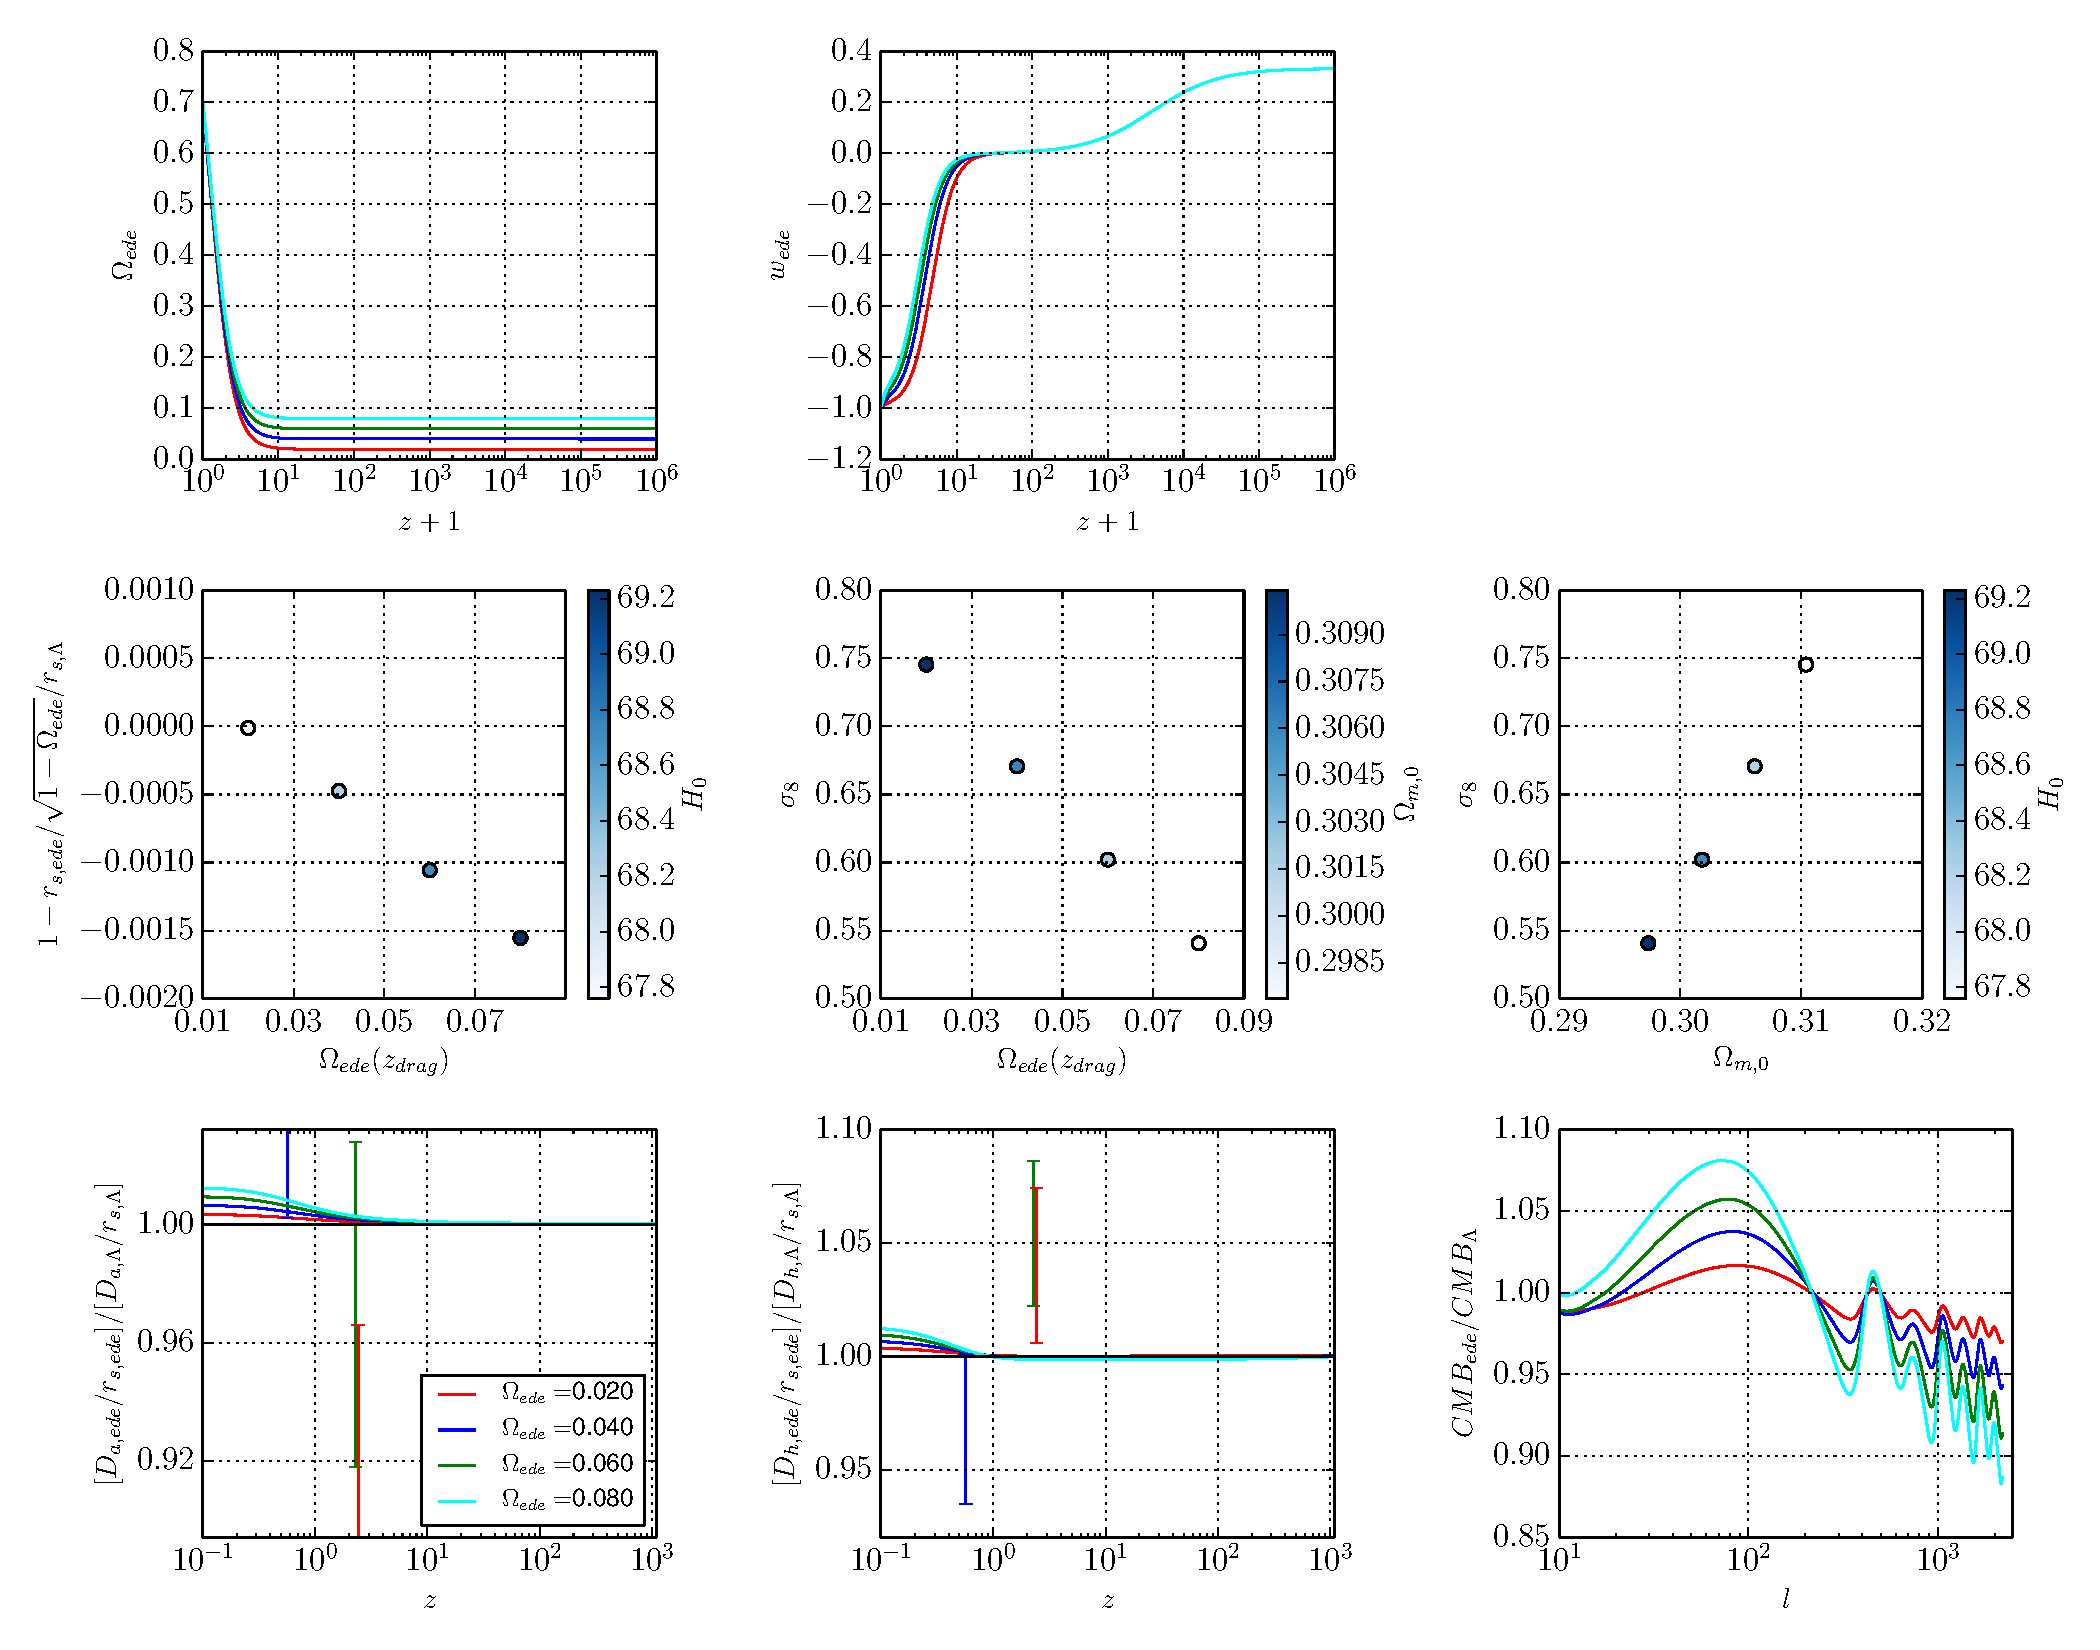
\includegraphics[trim = 2mm 2mm 3mm 1mm, clip, width=18cm, height=15cm ]{test_ede_Om.pdf}
  %\\
  % \includegraphics[scale=0.3 ]{Doran_cls}
  %  \includegraphics[scale=0.3 ]{Doran_cls2}
 \caption{Doran Model}
 \label{fig:fig1}
\end{figure*} 




%

We perform the same analysis as before: fix
 $\Omega_{m}h^2$  to the best fit values found
by Planck, and vary $H_0$ such that $D_A/r_s$ satisfies Planck constraints at the drag epoch.
%
From the figure, we notice that models with $\Omega_{ere} \sim 0.05$ satisfy Planck constraints (by construction),
and also provide a better fit for $D_H/r_d$ for BAO both galaxies and Lymann-$\alpha$, and a better fit, as well, for $D_A/r_s$
than the standard LCDM. Also for this particular model, we get a higher $H_0 \sim 75$ consistent with the Distance
ladder (Freedmann, Riess).

Planck values used throughout the calculations:  $\Omega_{b}h^2 = 0.02226$,  $\Omega_{c}h^2 =0.1193$, 
$H_0 = 67.51$, $A_{s} =2.1\times10^{-9}$, $n_{s}= 0.965$, and derived parameters 
$r_{zdrag}=147.42$, $100\theta_{zstar}=1.039706$, $\sigma_8 = 0.8194651 $.

\begin{figure}[h!]
\hspace*{-0.in}
  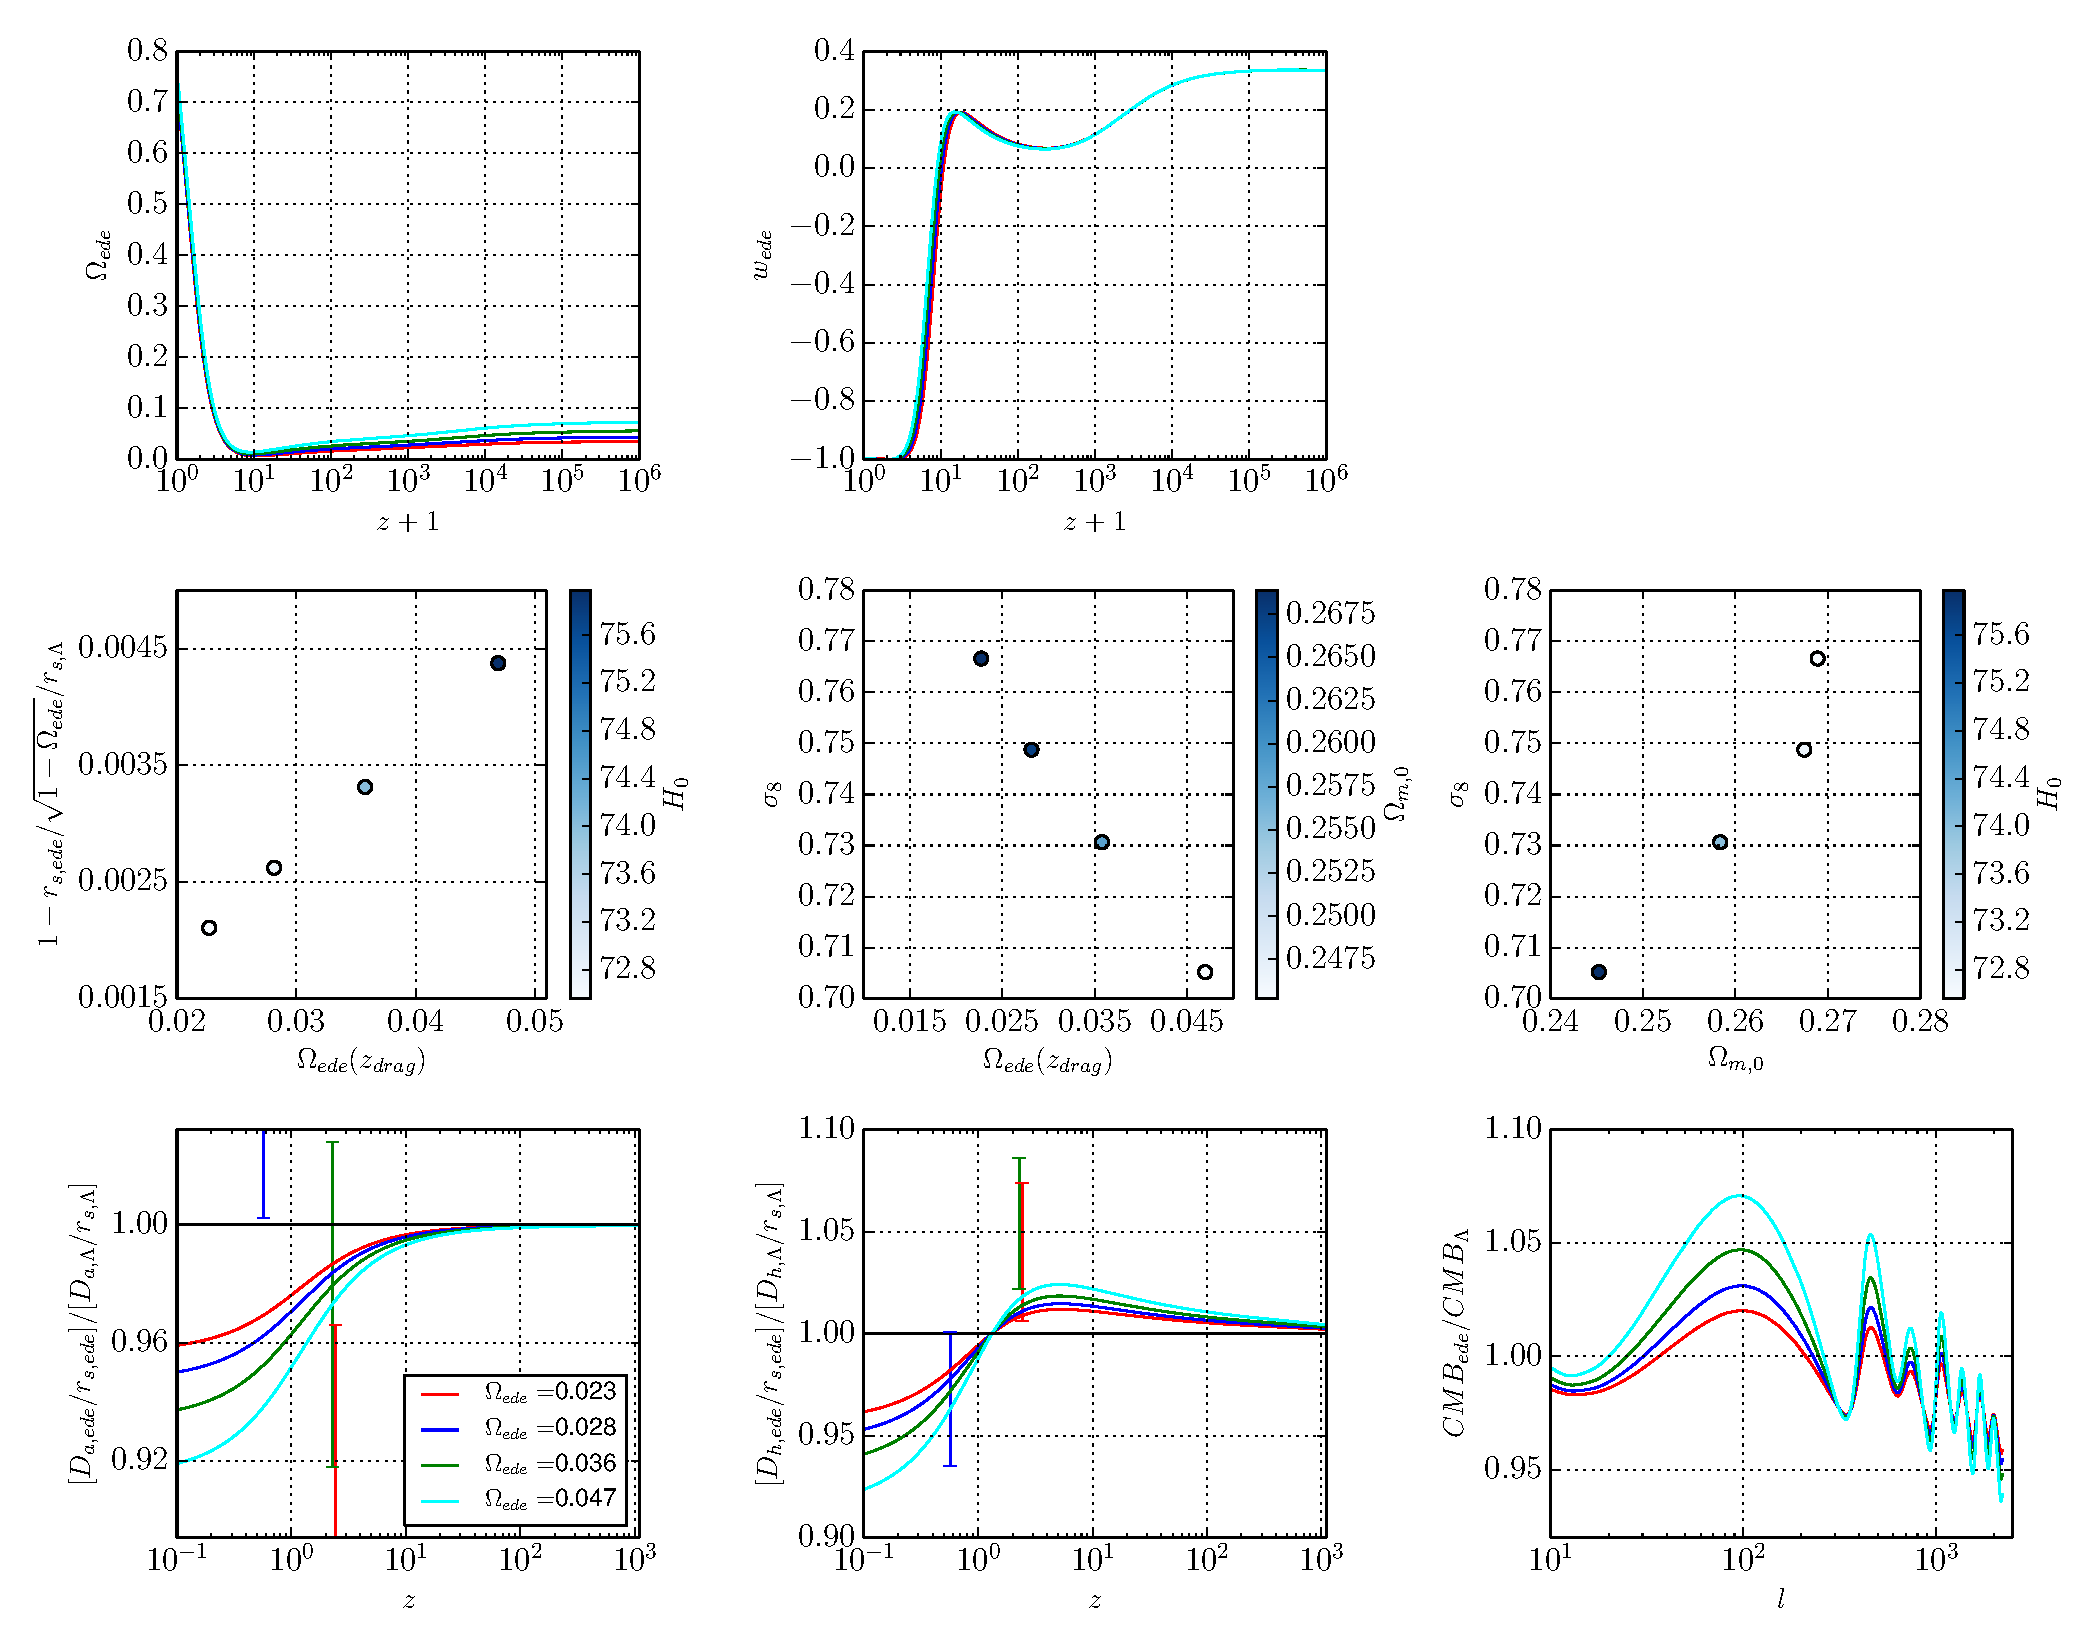
\includegraphics[trim = 2mm 2mm 3mm 1mm, clip, width=18cm, height=15cm]{test_quint_Om.pdf}
 \caption{Fix
 $\Omega_{m}h^2$  to the best fit values found
by Planck, and vary $H_0$ such that $D_A/r_s$ satisfies Planck constraints at the drag epoch, for five set of models 
in terms of $\{A, \lambda\}$. }
 \label{fig:fig1}
\end{figure} 

%\begin{figure}[h!]
%\hspace*{-0.9in}
%  \includegraphics[trim = 2mm 2mm 3mm 1mm, clip, width=18cm, height=12cm]{Dh_Da2}
% \caption{Same plot as the previous one, but the amplitude of the first peak is such that it matches in all models.}
% \label{fig:fig1}
%\end{figure} 

The Early Dark Energy model  provides and better fit to observations, compared to the $\Lambda$CDM model
and alleviate some tensions between datasets. $H_0$ is higher and $\Omega_m$ is lower, 
 matching observations of the distance ladder, and reducing the amplitude of low-redshift matter clustering
 by suppressing the growth of structure.
 
 
 \begin{figure*}[h!]
\hspace*{-0.in}
 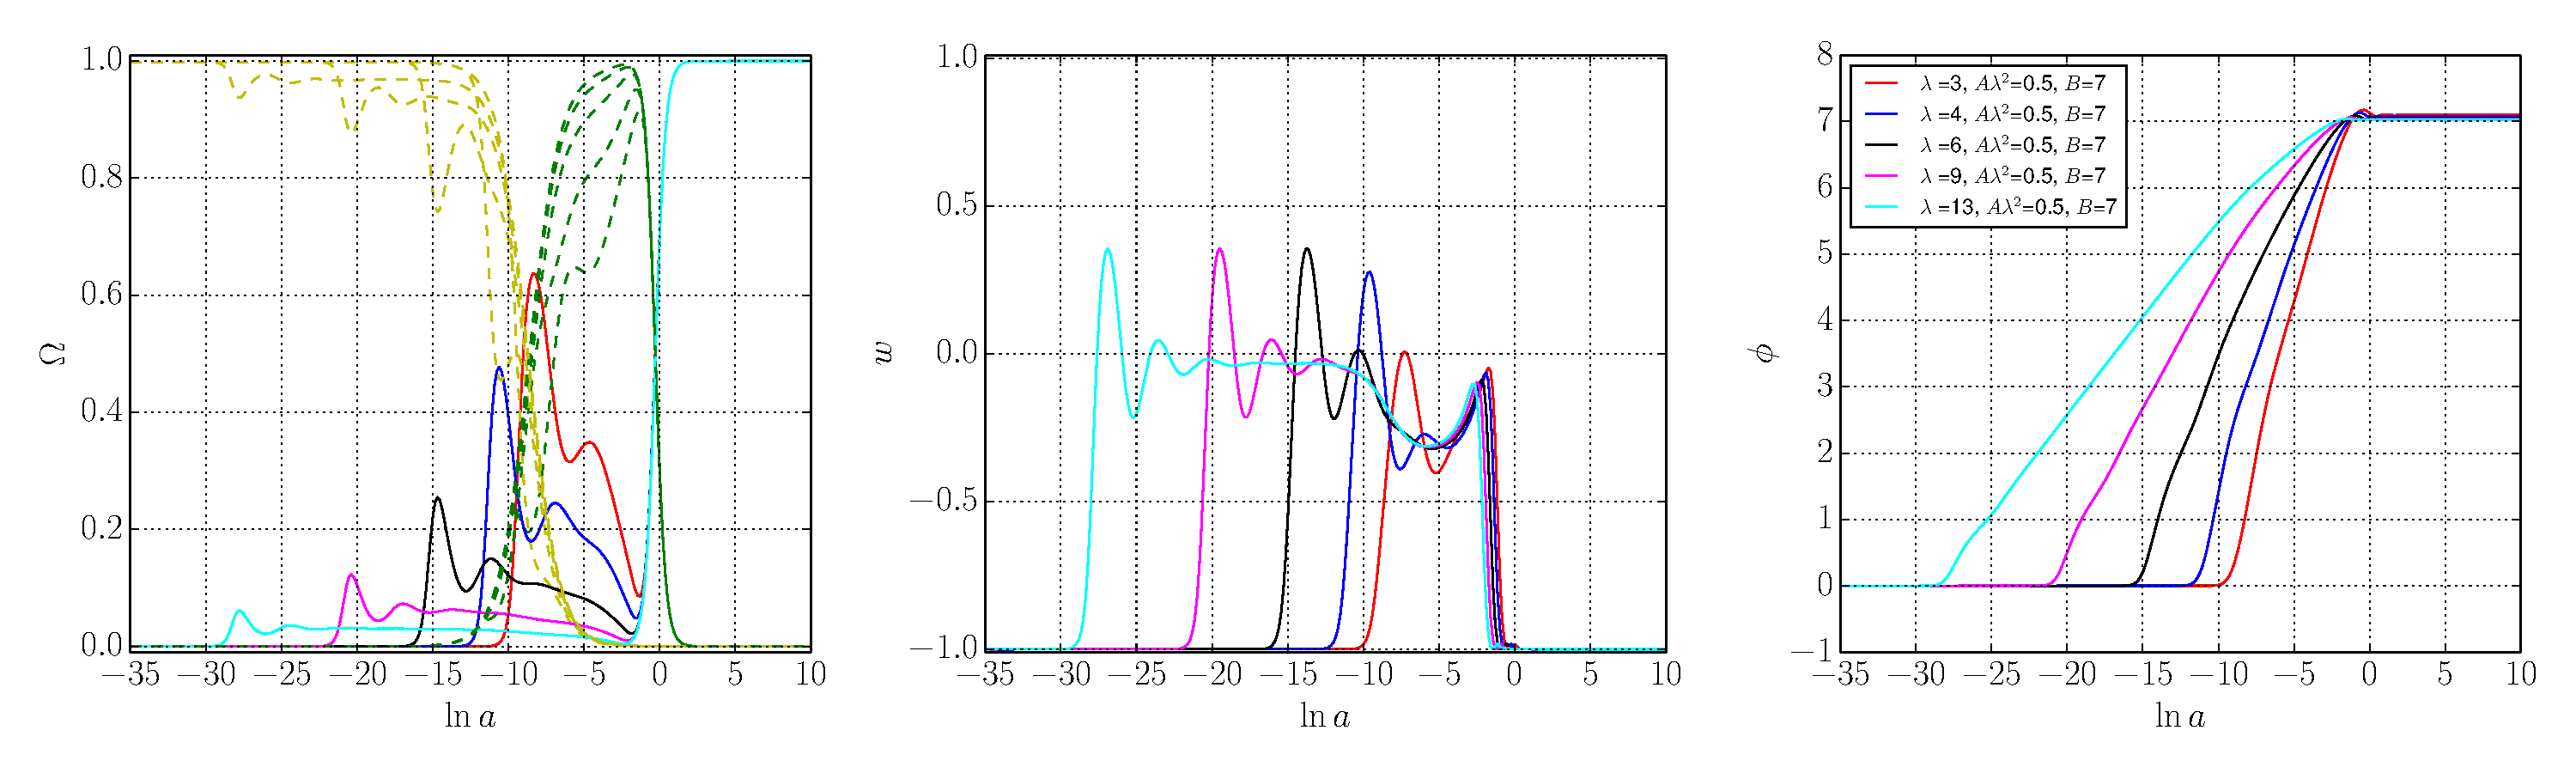
\includegraphics[scale=0.31]{Quintb_vl}\\
 \hspace*{-0.in}
  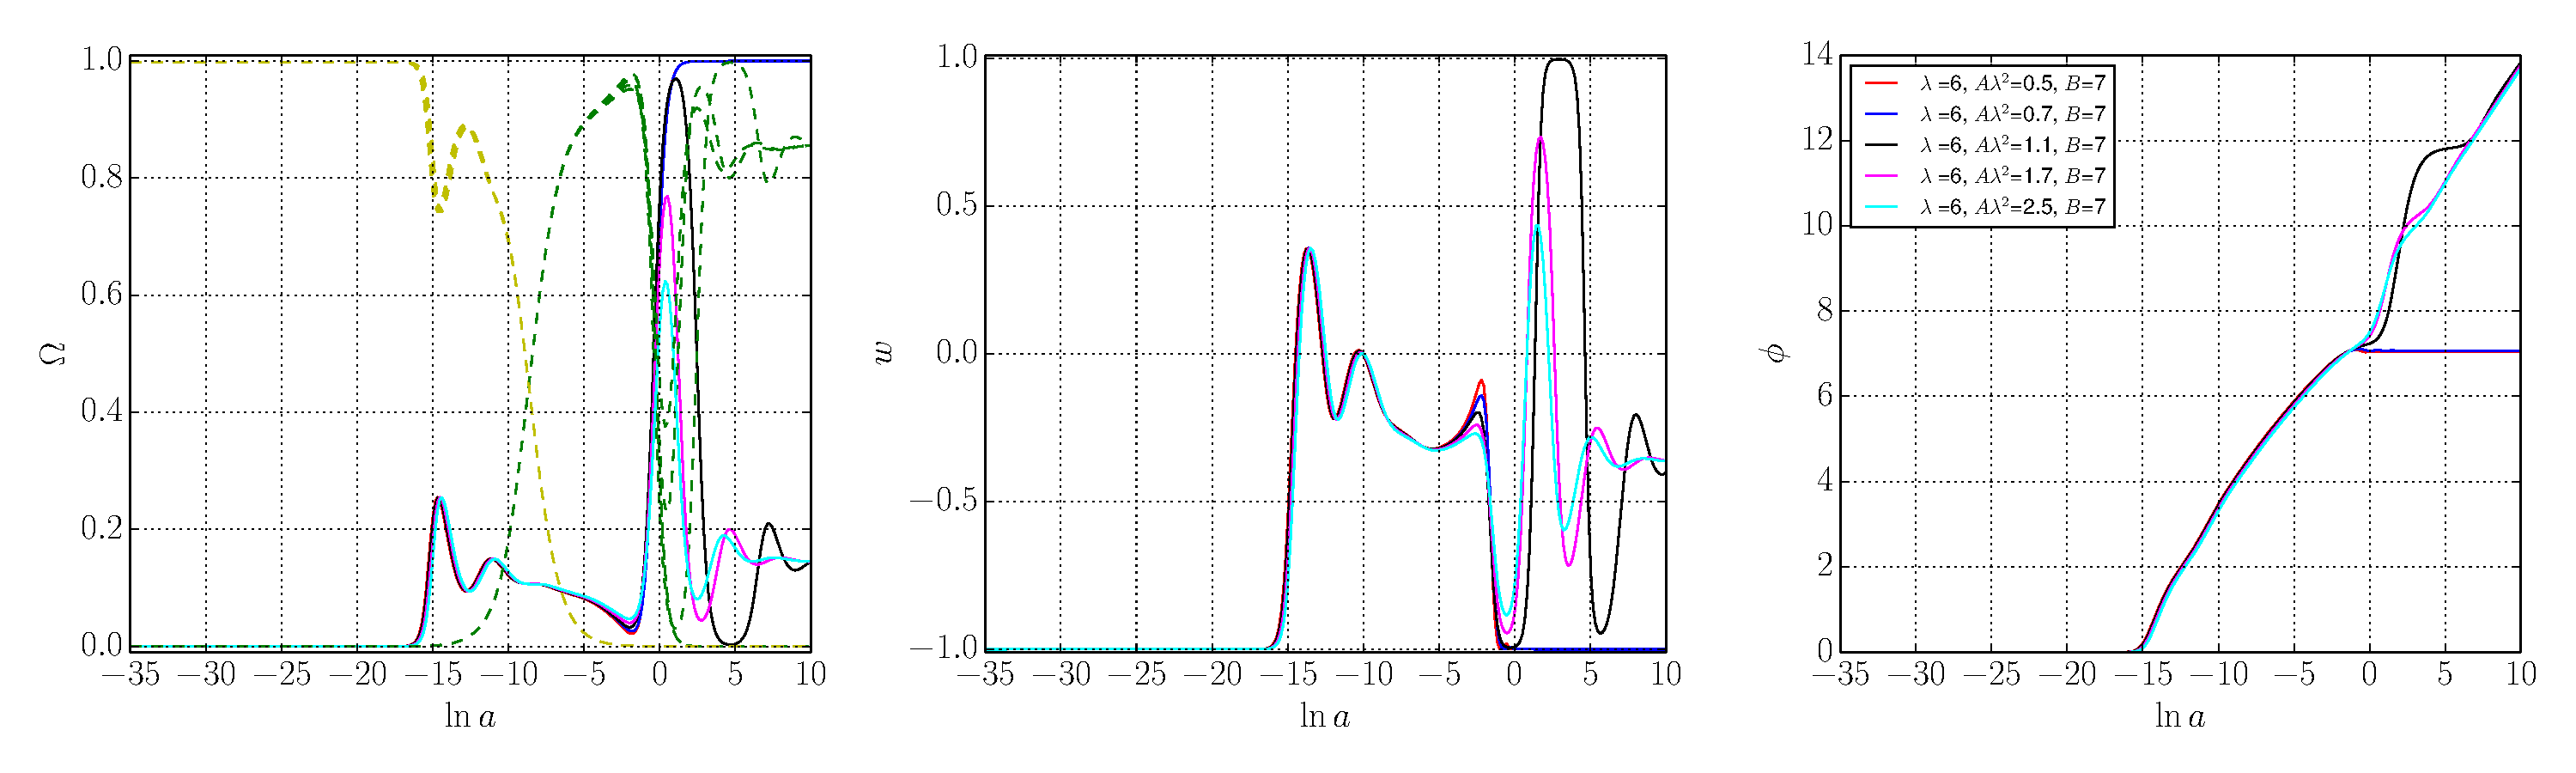
\includegraphics[scale=0.31]{Quintb_vAl}\\
  \hspace*{-0.in}
  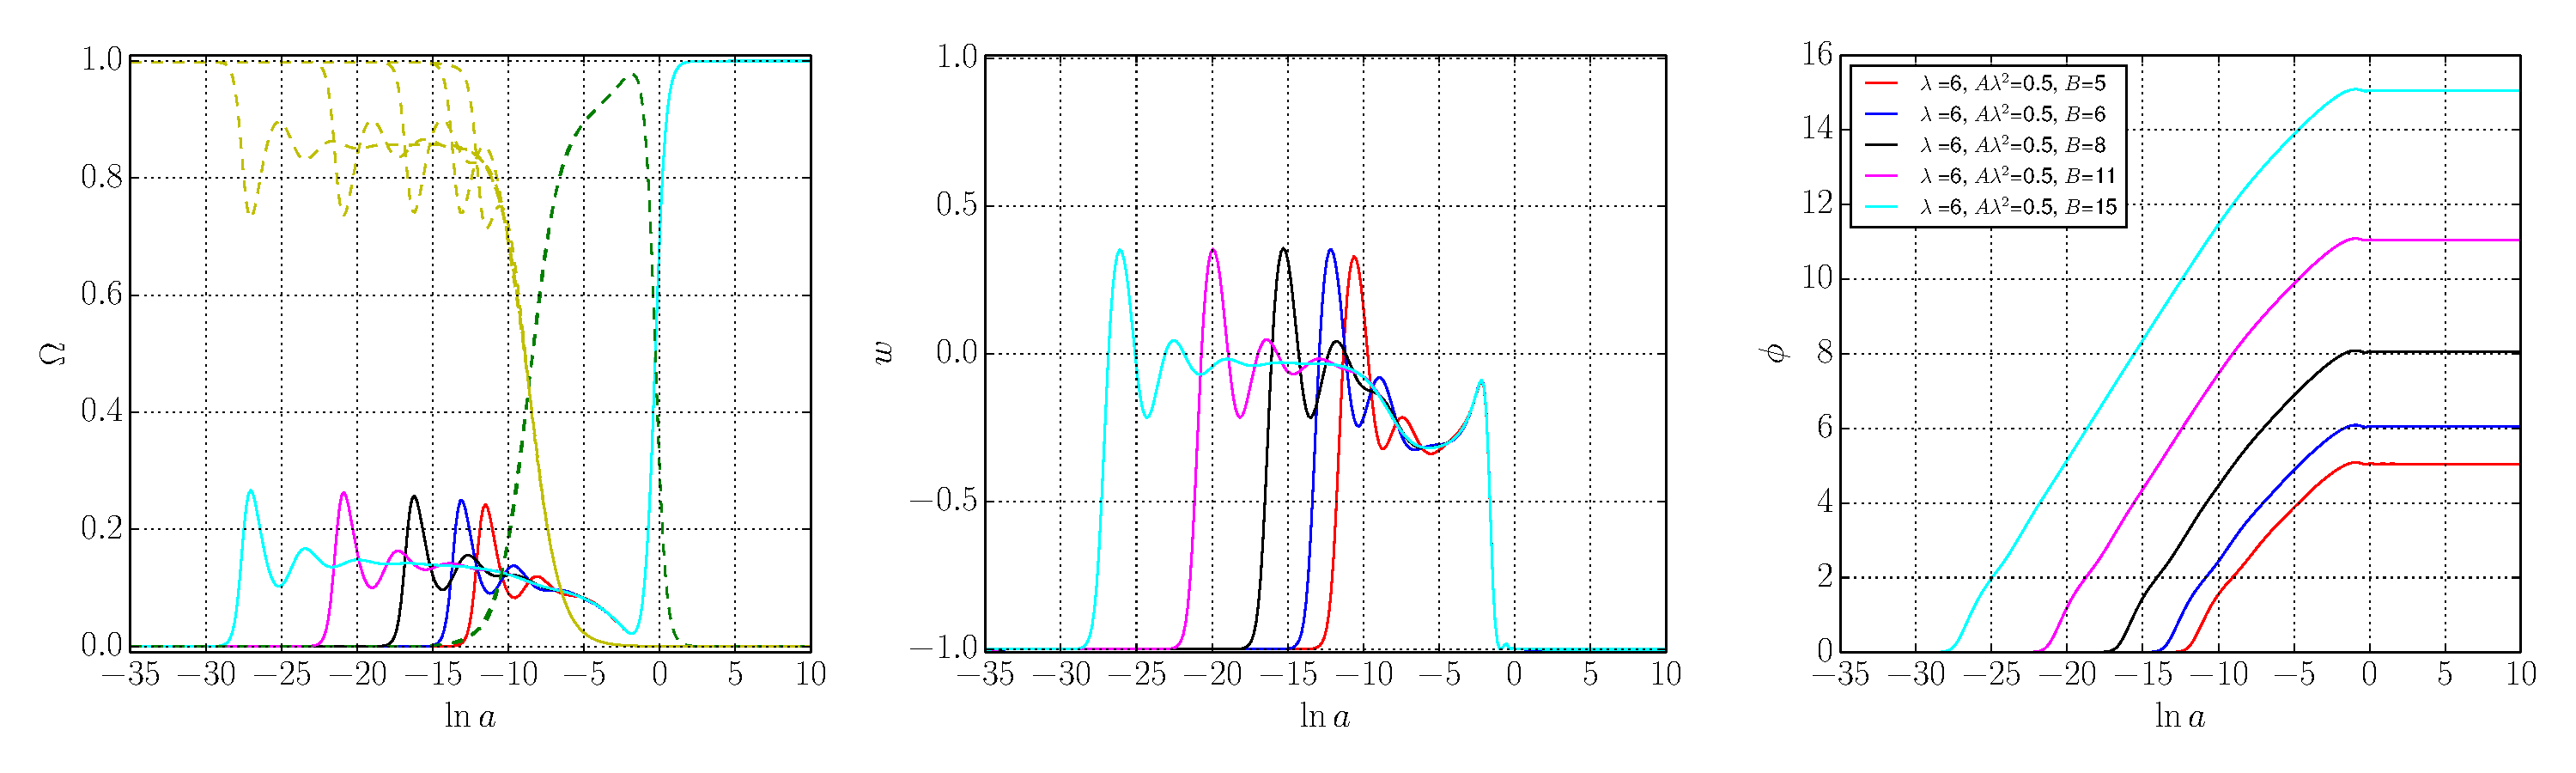
\includegraphics[scale=0.31]{Quintb_vB}\\
  % \hspace*{-1.in}
  %  \includegraphics[scale=0.34]{Quintb_vl2}
 \caption{  Three components of the universe: radiation (yellow), dark matter (green) 
 and Early Dark energy for different set of parameter combinations.
Density parameters (left), equation of state (middle) and the scalar
field (right) in terms of the $\ln(a)$ scale factor.
\as{Make sure these plots are actually readable. Can't see the labels
  at all!}
 }
 \label{fig:fig1}
\end{figure*} 

%\begin{figure}[h!]
%\hspace*{-0.9in}
%  \includegraphics[scale=0.45 ]{Dh_Da}
% \caption{$r_{s, LCDM}=149.01$ }
% \label{fig:fig1}
%\end{figure} 


%\begin{figure}[h!]
%\hspace*{1.in}
  %\includegraphics[scale=0.7 ]{Final}
 %\caption{$r_{s, LCDM}=149.01$ }
 %\label{fig:fig1}
%\end{figure} 

\end{document}

